%%
%% Author: jamie
%% 05/10/18
%%
\chapter{Agent Implementation}\label{ch:development}

\section{UCT Algorithm}\label{sec:MCTS}

\subsection{Tree Representation}\label{subsec:treeRepresentation}

\subsection{UCB Selection}\label{subsec:selection}

\subsection{Expansion}\label{subsec:expansion}

\subsection{Simulation}\label{subsec:simulation}

\subsection{Tree Update}\label{subsec:treeUpdate}

\subsection{Smooth UCT}\label{subsec:smoothUCT}

\section{Best Response Computation}\label{sec:bestResponseComputation}
In order to evaluate the performance of our agent we utilised exploitability as our primary metric.
Exploitability is a measure of how well our agent would fare against an opponent responding
optimally to our strategy.
Exploitability is related to the concept of Nash equilibria in that a Nash equilibrium
is induced by a strategy that cannot be exploited.

To calculate the exploitability of a strategy we must determine the best responses
to that strategy.
The first step in calculating the best response strategy involves
taking our agent's action selections and inserting them into the game tree\citep{heinrich2017reinforcement}.
In other words, wherever the agent must take an action in the game tree, we choose the best action
based on our MCTS estimations.
As such the resultant tree will consist of the MCTS player's decision nodes which will have
a single child node along with the second player's decision nodes and chance nodes
which will both have multiple children.
We can then evaluate the terminal states and propagate values back up the tree, with the highest
child value being propagated when we reach a decision node for player two and the average child
value being propagated for chance nodes.
This process will now be explained in detail with coding examples.

\subsection{Generating Best Response Tree}\label{subsec:applyMCTS}

\begin{figure}[ht]
    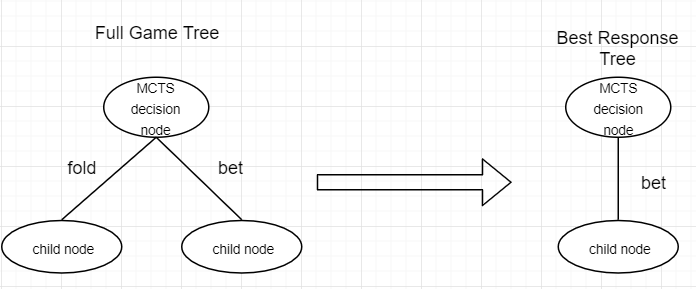
\includegraphics[scale=1]{images/best_response_tree_vs_full_tree.PNG}
    \caption{Generation of Best Response Tree}
\end{figure}

\subsection{Propagating Terminal Values}\label{subsec:propagateTerminals}
\subsection{Exploitability}\label{subsec:exploitability}